\documentclass[tikz,border=10pt]{standalone}
% Shared look for every TikZ diagram. Load with \input{../../tools/tikz-style.tex}
\usepackage[T1]{fontenc}
\usepackage{lmodern}
\renewcommand{\sfdefault}{lmr}  % diagrams use the same serif as the text
\usetikzlibrary{arrows.meta, positioning, shapes.geometric, calc, fit, backgrounds}
\definecolor{cblue}{HTML}{4C78A8}
\definecolor{corange}{HTML}{F58518}
\definecolor{cgreen}{HTML}{54A24B}
\definecolor{cred}{HTML}{E45756}
\definecolor{cpurple}{HTML}{B279A2}
\definecolor{cgrey}{HTML}{6B6B6B}
\tikzset{
  every picture/.style={font=\sffamily, line width=1.2pt},
  box/.style={draw=#1, fill=#1!12, rounded corners=4pt, align=center, inner sep=7pt, minimum height=1.1cm},
  box/.default=cgrey,
  arrow/.style={-{Stealth[length=3mm]}, draw=cgrey, line width=1.4pt},
  title/.style={font=\sffamily\bfseries\Large},
  note/.style={font=\sffamily\small, text=cgrey, align=center},
}
\AtBeginDocument{\hyphenpenalty=10000 \exhyphenpenalty=10000}

\begin{document}
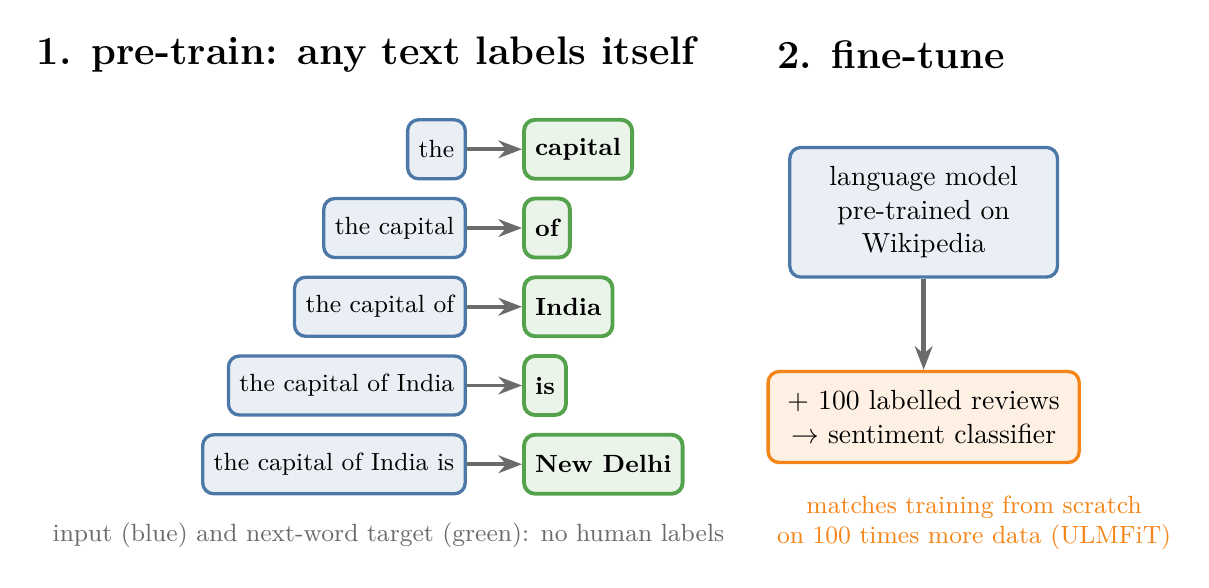
\begin{tikzpicture}[w/.style={box=cblue, inner sep=4pt, minimum height=0.75cm, font=\sffamily\small},
  t/.style={box=cgreen, inner sep=4pt, minimum height=0.75cm, font=\sffamily\small\bfseries}]
  \node[title, anchor=west] at (-0.2,1.2) {1. pre-train: any text labels itself};
  \foreach \ctx/\ans/\y in {{the}/{capital}/0, {the capital}/{of}/-1.0, {the capital of}/{India}/-2.0, {the capital of India}/{is}/-3.0, {the capital of India is}/{New Delhi}/-4.0} {
    \node[w, anchor=east] (c) at (5.4,\y) {\ctx};
    \draw[arrow] (c.east) -- ++(0.7,0) node[t, anchor=west] {\ans};
  }
  \node[note, anchor=west] at (0,-4.9) {input (blue) and next-word target (green): no human labels};
  \node[box=cblue, minimum width=3.4cm] (pt) at (11.2,-0.8) {language model\\pre-trained on\\Wikipedia};
  \node[title, anchor=west] at (9.2,1.2) {2. fine-tune};
  \node[box=corange, minimum width=3.4cm] (ft) at (11.2,-3.4) {+ 100 labelled reviews\\$\to$ sentiment classifier};
  \draw[arrow, line width=2pt] (pt) -- (ft);
  \node[note, anchor=west, text=corange] at (9.2,-4.75) {matches training from scratch\\on 100 times more data (ULMFiT)};
\end{tikzpicture}
\end{document}
